% Lecture Template for ME3023 -  Measurements in Mechanical Systems - Tennessee Technological University
% Spring 2020 - Summer 2020 - Fall 2020 - Spring 2021 - Summer 2021 - Fall 2023
% Tristan Hill, May 07, 2020 - June 12, 2020 - July 08, 2020 - Novemeber 02, 2020 - March 28, 2021 - May 25, 2021 - August 21, 2022 - September 02, 2023 - September 09, 2023 - March 24, 2024

% Fall 2023 - condensing and streamlining lectures by combining topics into a single PDF under the module name
%			  this will simplify file and link management as well as make lectures easier to use in class
%			- added image/ to clean directory and reduce redundancy, specific to module for now  

% Module Name: - Data Acquisition
% Topic 1 -
% Topic 2 -
% Topic 3 -


\documentclass[fleqn]{beamer} % for presentation (has nav buttons at bottom)

%\usepackage{/home/tntech.edu/thill/courses/measurements/lectures/measurements_lectures}
%\usepackage{/home/thill/courses/measurements/lectures/measurements_lectures}
\usepackage{/mnt/c/Users/thill/Documents/courses/measurements/lectures/measurements_lectures}

\author{ME3023 - Measurements in Mechanical Systems} 

\newcommand{\MNUM}{8\hspace{2mm}} % module number 
\newcommand{\moduletitle}{Data Acquisition}

\newcommand{\sectionItitle}{Analog to Digitial Conversion}
\newcommand{\sectionIItitle}{DAQ Hardware and Applications}
\newcommand{\sectionIIItitle}{Sampling and Aliasing}

\newcommand{\sectionIsubsectionItitle}{DAQ and Computer Storage}
\newcommand{\sectionIsubsectionIItitle}{Number Types}
\newcommand{\sectionIsubsectionIIItitle}{Analog to Digital Conversion and DAQ}
\newcommand{\sectionIsubsectionIVtitle}{Activity: ADC Resolution Calculation}

\newcommand{\sectionIIsubsectionItitle}{Signal Types and DAQ}
\newcommand{\sectionIIsubsectionIItitle}{EMI Considerations}
\newcommand{\sectionIIsubsectionIIItitle}{Available Hardware}
\newcommand{\sectionIIsubsectionIVtitle}{Software Integration}

\newcommand{\sectionIIIsubsectionItitle}{Sampling}
\newcommand{\sectionIIIsubsectionIItitle}{The Aliasing Phenomenon}
\newcommand{\sectionIIIsubsectionIIItitle}{Example by Hand}
\newcommand{\sectionIIIsubsectionIVtitle}{MATLAB Example}

 \newcommand{\btVFill}{\vskip0pt plus 1filll}

% custom box
\newsavebox{\mybox}

\title{Lecture Module - \moduletitle}

\date{Mechanical Engineering\vspc Tennessee Technological University}

\begin{document}

	\lstset{language=MATLAB,basicstyle=\ttfamily\small,showstringspaces=false}

	\frame{\titlepage \center\begin{framed}\Large \textbf{Module \MNUM - \moduletitle}\end{framed} \vspace{5mm}}

	% Module Outline
	\begin{frame} 
		\large \textbf{Module \MNUM - \moduletitle} \vspace{3mm}\\

		\begin{itemize}
			\item Topic 1 - \hyperlink{sectionI}{\sectionItitle} \vspc % section I
			\item Topic 2 - \hyperlink{sectionII}{\sectionIItitle} \vspc % section II
			\item Topic 3 - \hyperlink{sectionIII}{\sectionIIItitle} \vspc % section III
		\end{itemize}

	\end{frame}

	% section I
	\section{\sectionItitle}\label{sectionI}

		% section I Outline
		\begin{frame} 
			\large \textbf{Topic 1 - \sectionItitle} \vspace{3mm}\\

			\begin{itemize}
				\item \hyperlink{sectionIsubsectionI}{\sectionIsubsectionItitle} \vspc %  section I subsection I
				\item \hyperlink{sectionIsubsectionII}{\sectionIsubsectionIItitle} \vspc % section I subsection II
				\item \hyperlink{sectionIsubsectionIII}{\sectionIsubsectionIIItitle} \vspc % section I subsection III
				\item \hyperlink{sectionIsubsectionIV}{\sectionIsubsectionIVtitle} \vspc % section I subsection IV
			\end{itemize}
		\end{frame}
		
		% section I subsection I 
		\subsection{\sectionIsubsectionItitle}\label{sectionIsubsectionI}

			\begin{frame}
				\frametitle{\sectionIsubsectionItitle}

				A data acquisition system is the portion of a measurement system that \underline{\hspace{20mm}} and \underline{\hspace{20mm}} data. 

				\begin{multicols}{2}
				
\includegraphics[scale=.30]{images/cartesian_6x6_B.png} 
				

				\end{multicols}
				\btVFill
				\tiny{Image: T.Hill, Text: Theory and Design of Mechanical Measurements }
	
			\end{frame}

			\begin{frame}
				\frametitle{\sectionIsubsectionItitle}

		
			\end{frame}

		% section I subsection II
		\subsection{\sectionIsubsectionIItitle}\label{sectionIsubsectionII}

			\begin{frame}
				\frametitle{\sectionIsubsectionIItitle}\small
				\bigskip

				\begin{itemize}

					\item Integers 

						\begin{itemize}
							\item Binary
							\item Decimal
							\item Hexadecimal
						\end{itemize}

					\item Fixed Point 		

					\item Floating Point 



				\end{itemize}

				\btVFill
				

			\end{frame}

			\begin{frame}
				\frametitle{\sectionIsubsectionIItitle}\small
				\bigskip

				\begin{multicols}{2}
				\begin{tabular}{|r|r|r|} \hline
					Binary 	& Decimal 	& Hexadecimal \\ \hline
					0		& 0			& 0 		\\ \hline	
					1		& 1			& 1 		\\ \hline
					10		& 2			& 2 		\\ \hline
					11		& 3			& 3 		\\ \hline
					100		& 4			& 4 		\\ \hline
							& 5			& 5 		\\ \hline
							& 6			& 6 		\\ \hline
						    & 7			& 7 		\\ \hline
							& 8			& 8 		\\ \hline
							& 9			& 9 		\\ \hline
							& 10		& A 		\\ \hline
							& 11		& B 		\\ \hline
				\end{tabular}

				\begin{tabular}{|r|r|r|} \hline
					Binary 	& Decimal 	& Hexadecimal \\ \hline
							& 12		& C 		\\ \hline	
							& 13		& D 		\\ \hline
							& 14		& E 		\\ \hline
							& 15		& F 		\\ \hline
							& 16		&  		\\ \hline
							& 17		&  		\\ \hline
							& 18		&  		\\ \hline
							& 19		&  		\\ \hline
							& 20		&  		\\ \hline
							& 21		&  		\\ \hline
							& 22	    &  		\\ \hline
							& 23	    &  		\\ \hline
				\end{tabular}
				\end{multicols}

				\btVFill
				\tiny{some reference}		

			\end{frame}

			\begin{frame}
				\frametitle{\sectionIsubsectionIItitle} \small
				\bigskip

				\begin{multicols}{2}
				\begin{tabular}{|r|r|r|} \hline
					Binary 	& Decimal 	& Hex. \\ \hline
					0		& 0			& 0 		\\ \hline	
					1		& 1			& 1 		\\ \hline
					10		& 2			& 2 		\\ \hline
					11		& 3			& 3 		\\ \hline
					100		& 4			& 4 		\\ \hline
					& 			&  		\\ \hline
					& 			&  		\\ \hline
					& 			&  		\\ \hline
					& 			&  		\\ \hline
					& 			&  		\\ \hline
					& 		&  		\\ \hline
					& 		&  		\\ \hline
				\end{tabular}

				\begin{tabular}{|r|r|r|} \hline
					Binary\hspace{18mm} 	& Decimal 	& Hex. \\ \hline
					0		& 0			& 0 		\\ \hline	
					1		& 1			& 1 		\\ \hline
					10		& 2			& 2 		\\ \hline
					11		& 3			& 3 		\\ \hline
					100		& 4			& 4 		\\ \hline
					& 			&  		\\ \hline
					& 			&  		\\ \hline
					& 			&  		\\ \hline
					& 			&  		\\ \hline
					& 			&  		\\ \hline
					& 		&  		\\ \hline
					& 		&  		\\ \hline
				\end{tabular}
				\end{multicols}

				\btVFill
				\tiny{some reference}	


			\end{frame}


			\begin{frame}

				\frametitle{\sectionIsubsectionIItitle} \small
				\bigskip




			  	Standard storage of a floating point value in memory\\	

			  	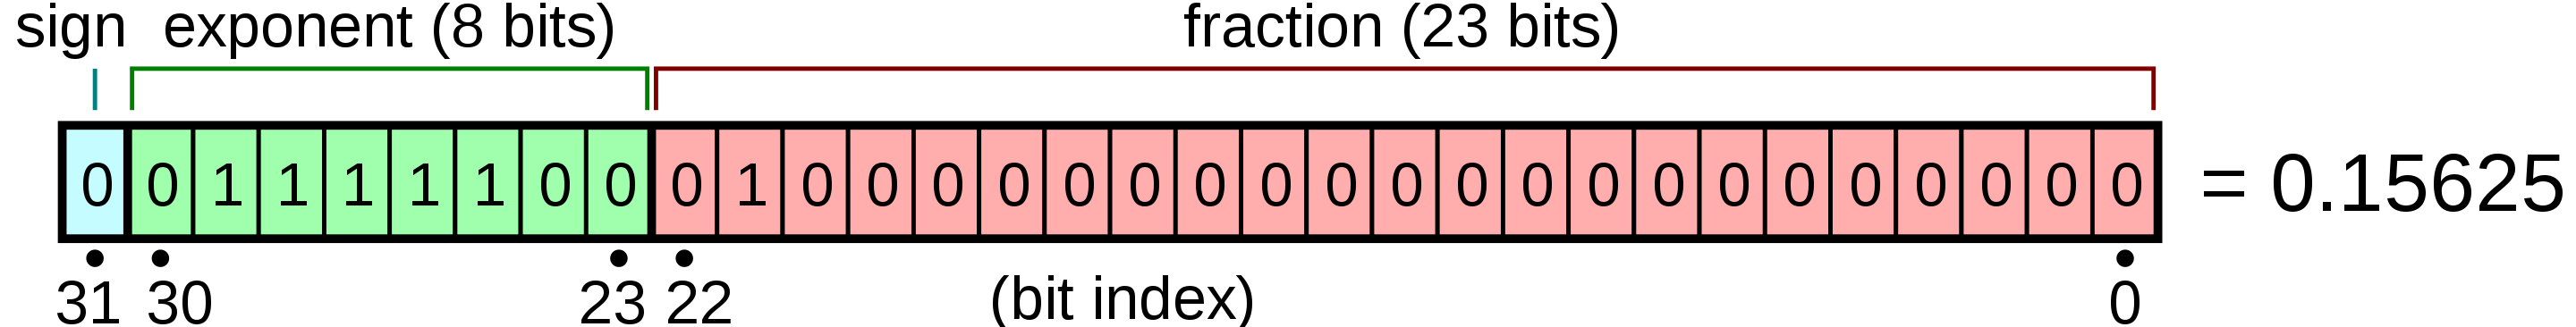
\includegraphics[scale=.10]{images/ieee754_bits.png}	
			  	\btVFill
				
				{\tiny \href{https://en.wikipedia.org/wiki/IEEE_754}{Wikipedia: IEEE Float} \href{https://en.wikipedia.org/wiki/Fixed-point_arithmetic}{Wikipedia: Fixed Point} }

			\end{frame}

			\begin{frame}
			\bigskip 


			
			\btVFill
			\tiny{Text: Theory and Design for Mechanical Measurements}	
			\end{frame}

			\begin{frame}

				\frametitle{\sectionIsubsectionIItitle} \small
				\bigskip

				\begin{multicols}{3}
					\underline{Integer} \vspace{10mm}\\
					Pros:\vspace{10mm}\\
					Cons:\vspace{10mm}\\
					Examples:

					\underline{Floating Point} \vspace{10mm}\\	
					Pros:\vspace{10mm}\\
					Cons:\vspace{10mm}\\
					Examples:

					\underline{Fixed Point} \vspace{10mm}\\	
					Pros:\vspace{10mm}\\
					Cons:\vspace{10mm}\\
					Examples:
				\end{multicols}
				
				\btVFill
				\tiny{Text: Theory and Design for Mechanical Measurements}	
			\end{frame}


		% section I subsection III
		\subsection{\sectionIsubsectionIIItitle}\label{sectionIsubsectionIII}
			\begin{frame} 
				\frametitle{\sectionIsubsectionIIItitle} \scriptsize

				\bigskip
				
				In electronics, an \underline{\hspace{20mm}} (ADC, A/D, or A-to-D) is a system that converts an analog signal, such as a sound picked up by a microphone or light entering a digital camera, into a digital signal. An ADC may also provide an isolated measurement such as an electronic device that converts an analog input voltage or current to a digital number representing the magnitude of the voltage or current. Typically the digital output is a two's complement binary number that is proportional to the input, but there are other possibilities.

				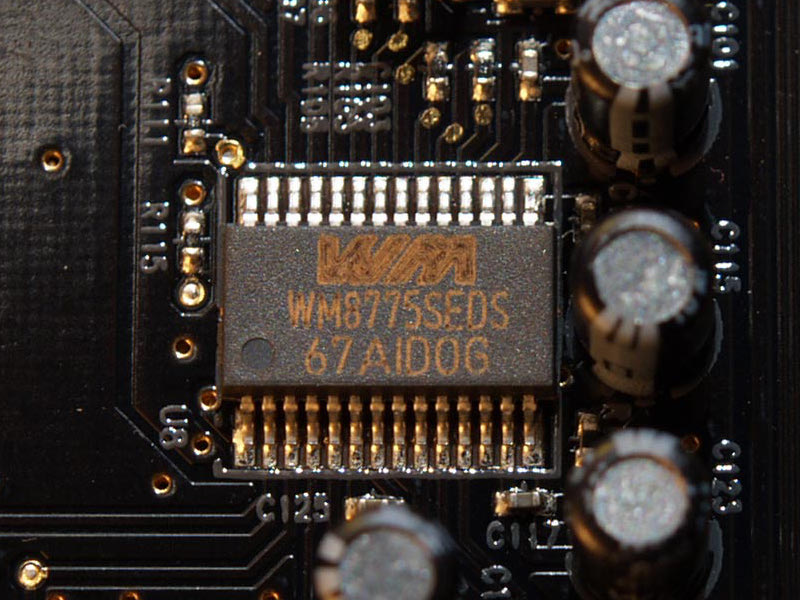
\includegraphics[scale=.15]{images/WM_WM8775SEDS-AB.jpg} \hspace{5mm} 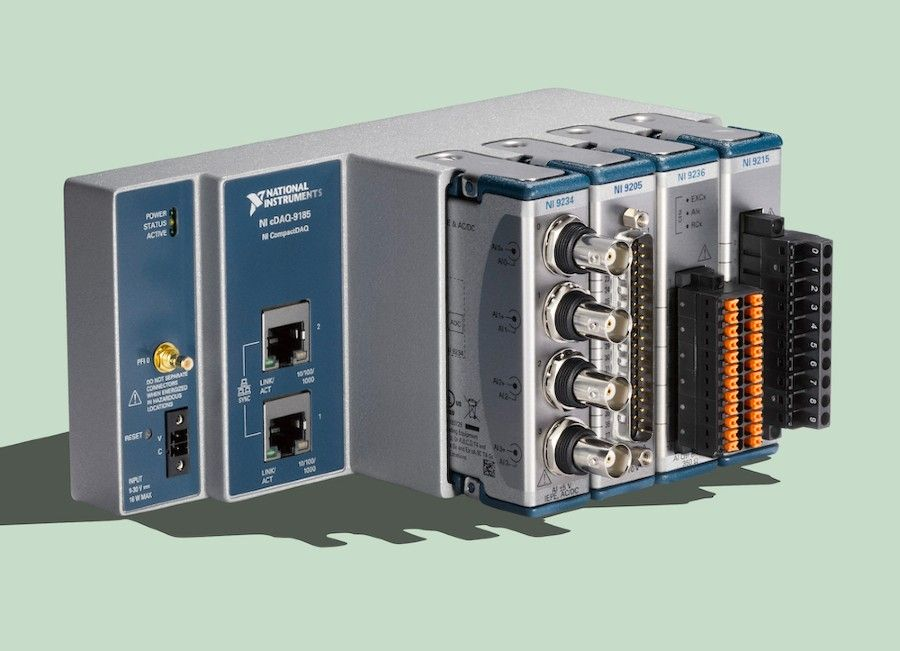
\includegraphics[scale=.15]{images/ni_cdaq.jpg}

				\btVFill
				\tiny{\href{https://en.wikipedia.org/wiki/Analog-to-digital_converter}{wikipedia,} \href{https://en.wikipedia.org/wiki/Analog-to-digital_converter\#/media/File:WM_WM8775SEDS-AB.jpg}{image} }	
			\end{frame}	

			\begin{frame} 
				\frametitle{\sectionIsubsectionIIItitle}

				
			\end{frame}	

		% section I subsection IV
		\subsection{\sectionIsubsectionIVtitle}\label{sectionIsubsectionIV}	

			\begin{frame}
				\frametitle{\sectionIsubsectionIVtitle} \scriptsize
				\bigskip

				It is important to realize the potential for \underline{\hspace{20mm}} resulting in a reduced quality measurement based on the parameters of the analog to digital conversion process. This issue can occur when designing systems around a \underline{\hspace{20mm}} analog to digital converter as well as when using \underline{\hspace{20mm}} DAQ equippment.  

				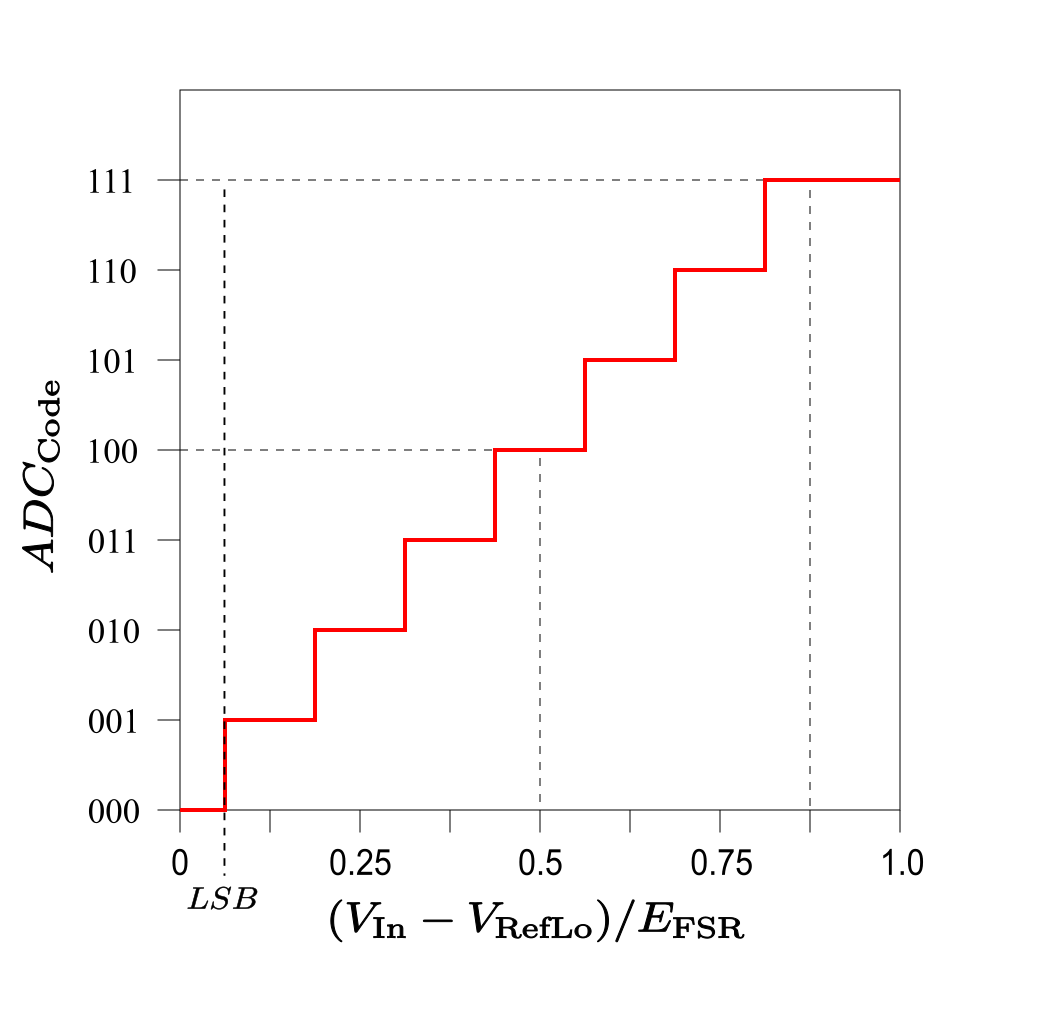
\includegraphics[scale=.2]{images/ADC_voltage_resolution.png}

				\btVFill
				\tiny{some reference}	

			\end{frame}

			\begin{frame}
				\frametitle{\sectionIsubsectionIVtitle}

				\bigskip


				\btVFill
				\tiny{: Theory and Design for Mechanical Measurements}
										
			\end{frame}

	
	% Section II
	\section{\sectionIItitle}\label{sectionII}

		% section II Outline
		\begin{frame}
			\large \textbf{Topic 2 - \sectionIItitle} \vspace{3mm}\\

			\begin{itemize}
				\item \hyperlink{sectionIIsubsectionI}{\sectionIIsubsectionItitle} \vspc %  section II subsection I
				\item \hyperlink{sectionIIsubsectionII}{\sectionIIsubsectionIItitle} \vspc % section II subsection II
				\item \hyperlink{sectionIIsubsectionIII}{\sectionIIsubsectionIIItitle} \vspc % section II subsection III
				\item \hyperlink{sectionIIsubsectionIV}{\sectionIIsubsectionIVtitle} \vspc % section II subsection IV
			\end{itemize}

		\end{frame}

		% section II subsection I
		\subsection{\sectionIIsubsectionItitle}\label{sectionIIsubsectionI}

			\begin{frame}[label=sectionIIsubsectionI]
				\frametitle{\sectionIIsubsectionItitle} \scriptsize

				\bigskip	

				{\it Most} data acquisition devices and systems \underline{\hspace{20mm}} and \underline{\hspace{20mm}} {\BL analog} voltage signals and possibly additional signal types. Signal \underline{\hspace{20mm}} may also be a feature on some systems. \vspace{5mm}\\

				A voltage signal requires a {\bf common} reference or \underline{\hspace{20mm}}.	\vspace{2mm}\\

				Signal Sources:
				\begin{itemize}
					\item Grounded or Ground-Referenced	\vspace{2mm}\\

					\item Ungrounded or Floating \vspace{2mm}\\		

				\end{itemize}	
				\vspace*{5mm}

				Measurement (DAQ) Systems:
				\begin{itemize}
					\item Common Ground \vspace{2mm}\\

					\item Common Mode Voltage \vspace{2mm}\\

					\item Isolated Ground \vspace{2mm}\\

				\end{itemize}
				

				\btVFill
				\tiny{\href{https://www.ni.com/en/support/documentation/supplemental/06/grounding-considerations---intermediate-analog-concepts.html}{NI},}
				\tiny{\href{https://digilent.com/reference/daq-and-datalogging/documents/analog-input-signal-connections-1}{Digilent}}

				\btVFill
				\tiny{Text: Theory and Design for Mechanical Measurements}
		
			\end{frame}

		    \begin{frame}[label=sectionIIsubsectionI]
				\frametitle{\sectionIIsubsectionItitle} \scriptsize

				{\it Most} data acquisition devices and systems measure and record {\BL analog} voltage signals and possibly additional signal types. Signal {\GR generation} may also be a feature on some systems. \vspace{5mm}\\

					%\begin{multicols}{2}
					2 Major Configurations:
					\begin{itemize}
						\item
						\underline{Single-Ended Signals} \vspace{0mm}\\
						The signal is measured as a voltage between a \underline{\hspace{20mm}} conductor and the \underline{\hspace{20mm}} which must be carried on a separate conductor or wire. \vspace{10mm}\\
					
						\item
						\underline{Double-Ended (Differential) Signals} \vspace{0mm}\\			
						The signal is measured as the {\PN difference} between \underline{\hspace{20mm}} voltages ({\PN double}) carried on separate conductors, or wires. Typically a \underline{\hspace{20mm}} is shared between the two devices requiring a third conductor. 
					\end{itemize}
				
					%\end{multicols}
					\btVFill
					\tiny{Read more here: \href{https://www.mccdaq.com/TechTips/TechTip-4.aspx}{MCCDAQ}}

			\end{frame}	

			 \begin{frame}[label=sectionIIsubsectionI]
				\frametitle{\sectionIIsubsectionItitle} \scriptsize

				\begin{multicols}{2}
					\underline{Single-Ended Signals} \vspace{10mm}\\
					
					Pros:\vspace{10mm}\\
					Cons:\vspace{10mm}\\
					Examples:
					
					\underline{Double-Ended Signals} \vspace{10mm}\\
					
					Pros:\vspace{10mm}\\
					Cons:\vspace{10mm}\\
					Examples:
					
					
				\end{multicols}
				\btVFill
				\tiny{Text: Theory and Design for Mechanical Measurements}
			\end{frame}


		% section II subsection II
		\subsection{\sectionIIsubsectionIItitle}\label{sectionIIsubsectionII}

			\begin{frame}
				\frametitle{\sectionIIsubsectionIItitle} \scriptsize
				\bigskip

				\underline{\hspace{20mm}}, also called radio-frequency interference (RFI) when in the radio frequency spectrum, is a disturbance generated by an external source that affects an electrical circuit by electromagnetic induction, electrostatic coupling, or conduction. \vspace{5mm}\\


				A {\it combination} of naturally occuring and human made sources of interference is always present. The total EMI affecting a system is determined by the local conditions as well as global environmental influences. \vspace{5mm}\\


				Sources of EMI:
				\begin{itemize}

					\item 
					\item  
					\item 
					\item 
					\item 

				\end{itemize}


				\btVFill
				\tiny{\href{https://csrc.nist.gov/glossary/term/electromagnetic_interference}{NIST}}		
			\end{frame}

		% section II subsection II
		\subsection{\sectionIIsubsectionIItitle}\label{sectionIIsubsectionII}

			\begin{frame}
				\frametitle{\sectionIIsubsectionIItitle} \scriptsize
	
				\bigskip

				In data acquisition, electromagnetic interference (EMI) can cause \underline{\hspace{20mm}} of signal quality and data \underline{\hspace{20mm}} in the form of \underline{\hspace{20mm}} and or \underline{\hspace{20mm}}. \vspace{10mm}

				Consider the case of an analog signal transmitted from a sensor to a DAQ device. What can be done to avoid issues associated with EMI?  \vspace{5mm}\\

				Methods of reducing EMI affects:
				\begin{itemize}
					\item Proximity - 

					\item Differential signal - 

					\item Noise rejection cables/wires -

				\end{itemize}


				\btVFill
				\tiny{\href{https://en.wikipedia.org/wiki/Twisted_pair}{wikipedia: twisted pair,}\href{https://www.mouser.com/pdfdocs/alphawire-Understanding-Shielded-Cable.pdf}{Mouser-Alphawire}}		
			\end{frame}

		% section II subsection III
		\subsection{\sectionIIsubsectionIIItitle}\label{sectionIIsubsectionIII}

			\begin{frame}
				\frametitle{\sectionIIsubsectionIIItitle} 

				\bigskip

				\begin{itemize}
					
					\item National Instruments \vspace{6mm}\\
					
					\item Measurement Computing  \vspace{6mm}\\
					
					\item dSPACE  \vspace{6mm}\\
					
					\item Arduino or other 
					
				\end{itemize}

				\btVFill
				\tiny{ : Theory and Design for Mechanical Measurements}

			\end{frame}

			\begin{frame}
				\frametitle{\sectionIIsubsectionIIItitle}

				\bigskip

				\begin{itemize}
					\item National Instruments \vspace{6mm}\\
					
					\item Measurement Computing  \vspace{6mm}\\
					
					\item dSPACE  \vspace{6mm}\\
					
					\item Arduino or other 
					
				\end{itemize}

				\btVFill
				\tiny{: Theory and Design for Mechanical Measurements}	
			
			\end{frame}

			\begin{frame}
			\frametitle{\sectionIIsubsectionIIItitle}




				\btVFill
				\tiny{ : Theory and Design for Mechanical Measurements}	

			\end{frame}

		% section II subsection IV 
		\subsection{\sectionIIsubsectionIVtitle}\label{sectionIIsubsectionIV}

			\begin{frame}
				\frametitle{\sectionIIsubsectionIVtitle}


			\end{frame}

			\begin{frame}
				\frametitle{\sectionIIsubsectionIVtitle}


			\end{frame}
		
	% Section III
	\section{\sectionIIItitle}\label{sectionIII}

		% section III Outline
		\begin{frame}
			\large \textbf{Topic 3 - \sectionIIItitle} \vspace{3mm}\\

			\begin{itemize}
				\item \hyperlink{sectionIIIsubsectionI}{\sectionIIIsubsectionItitle} \vspc %  section III subsection I
				\item \hyperlink{sectionIIIsubsectionII}{\sectionIIIsubsectionIItitle} \vspc % section III subsection II
				\item \hyperlink{sectionIIIsubsectionIII}{\sectionIIIsubsectionIIItitle} \vspc % section III subsection III
				\item \hyperlink{sectionIIIsubsectionIV}{\sectionIIIsubsectionIVtitle} \vspc % section III subsection IV
			\end{itemize}

		\end{frame}

		% section III subsection I
		\subsection{\sectionIIIsubsectionItitle}\label{sectionIIIsubsectionI}

			\begin{frame}
				\frametitle{\sectionIIIsubsectionItitle}

				\bigskip
						...
				A discrete time signal usually
				results from the \underline{\hspace{20mm}} of a continuous variable at \underline{\hspace{20mm}} finite time intervals.
				...	
				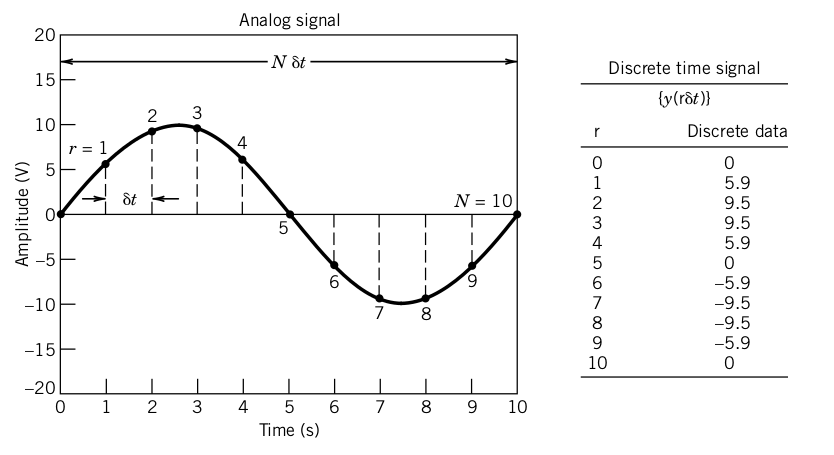
\includegraphics[scale=.3]{images/sampling_fig7_1.png}
			
				\btVFill
				\tiny{Text,Figure: Theory and Design for Mechanical Measurements Ch. 7}

			\end{frame}

			\begin{frame}
				\frametitle{\sectionIIIsubsectionItitle}
		
			\end{frame}

		% section III subsection II
		\subsection{\sectionIIIsubsectionIItitle}\label{sectionIIIsubsectionII}	

			\begin{frame}
				\frametitle{\sectionIIIsubsectionIItitle}

				\bigskip
				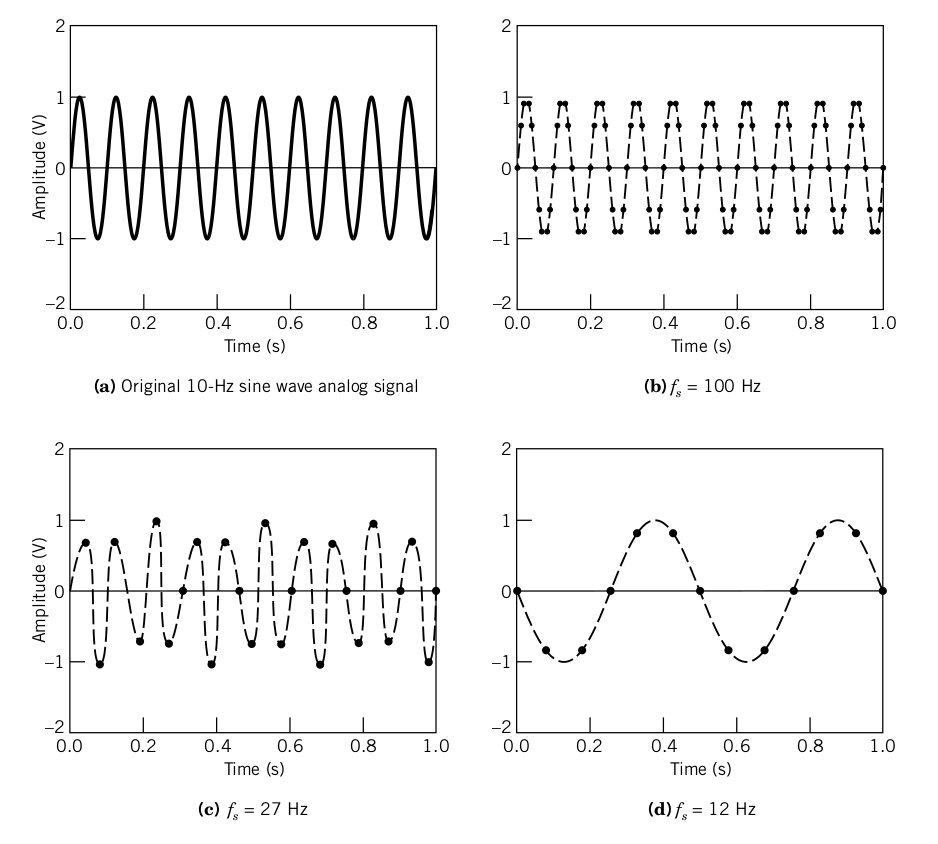
\includegraphics[scale=.2]{images/aliasing_fig7_2.png}


				\btVFill
				\tiny{Figure: Theory and Design for Mechanical Measurements Ch. 7}		

			\end{frame}

		% section III subsection III
		\subsection{\sectionIIIsubsectionIItitle}\label{sectionIIIsubsectionIII}

			\begin{frame}
				\frametitle{\sectionIIIsubsectionIIItitle}

				\bigskip
				
\includegraphics[scale=.35]{images/cartesian_6x12.png}


				\btVFill
				\tiny{Image: T.Hill}

			\end{frame}

			\begin{frame}
				\frametitle{\sectionIIIsubsectionIIItitle}



			\end{frame}

		% section III subsection IV
		\subsection{\sectionIIIsubsectionIVtitle}\label{sectionIIIsubsectionIV}	

			\begin{frame}[containsverbatim]
				\frametitle{\sectionIIIsubsectionIVtitle}\scriptsize

				\begin{lstlisting}
				% ME3023 - Tennessee Technological University 
				% Tristan Hill - October 10, 2019 - April 14, 2021
				% Data Acquisition Topic 3 - Sampling and Aliasing

				clear variables; close all; clc

				% simulate a continuous signal
				A1=5; f1=3;
				w1=2*pi*f1;

				dt_sim=0.001; t_stop=6;
				t_sim=0:dt_sim:t_stop;
				y_sim=A1*sin(w1*t_sim);
				\end{lstlisting}

			\end{frame}

			\begin{frame}[containsverbatim]
				\frametitle{\sectionIIIsubsectionIVtitle}\scriptsize
				
				\begin{lstlisting}

				% simulate sampling the signal
				dt_sam = 0.3;
				t_sam=0:dt_sam:t_stop;
				y_sam=A1*sin(w1*t_sam);

				% show the figure
				figure(1); hold on
				plot(t_sim,y_sim,'-',t_sam,y_sam,'o')
				axis([0 t_stop -1.2*A1 1.2*A1])
				grid on
				\end{lstlisting}


			
				\tiny{MATLAB code: T. Hill}	

			\end{frame}

\end{document}





